\documentclass[conference,letterpaper]{IEEEtran}
\IEEEoverridecommandlockouts
\usepackage[T1]{fontenc}
\usepackage{newtxtext,newtxmath}
\usepackage{graphicx}
\usepackage{booktabs}
\usepackage{multirow}
\usepackage{amsmath}
\usepackage{xcolor}
\usepackage{tikz}
\usetikzlibrary{positioning,arrows.meta,calc,fit,backgrounds}
\usepackage[hidelinks]{hyperref}
\usepackage[capitalise,nameinlink]{cleveref}
\usepackage{microtype}

\definecolor{vblue}{HTML}{2a78d6}
\definecolor{vorange}{HTML}{eb6834}
\definecolor{vaqua}{HTML}{1baf7a}
\definecolor{vgray}{HTML}{8a8984}
\definecolor{vink}{HTML}{52514e}

\newcommand{\pp}{\,pp}
\newcommand{\ci}[2]{\mbox{$[#1,\,#2]$}}
\newcommand{\cond}[1]{\textsf{\small #1}}
\crefname{figure}{Fig.}{Figs.}
\crefname{table}{Table}{Tables}
\crefname{section}{Sec.}{Secs.}

\begin{document}

\title{Where Is the Object in the Giver's Hand?\\ Geometric Coordination and Residual Reinforcement Learning for Robust Bimanual Handover}

\author{\IEEEauthorblockN{Yan Wen}
\IEEEauthorblockA{CSCI 645 Robot Manipulation, Fall 2026\\
University of Southern California}}

\maketitle

\begin{abstract}
In a handover, the receiving gripper must grasp an object whose pose is set by another gripper's grasp. Errors
in that pose cause misaligned grasps, and errors in release timing cause drops. We ask when a learned residual
policy improves a training-free geometric controller for this task, and what information the controller needs
when the object is not where it assumes. We build a two-arm Franka handover of a rigid bar in Isaac Lab with
parallel-jaw grippers. A geometric module aligns the receiver to the estimated grasp point, anchors shared holding
and gates the giver's release on stable receiver contact. A PPO residual adds bounded Cartesian corrections. We test
four uncertainty regimes with preregistered, held-out evaluations and paired bootstrap statistics: pose and timing
perturbations, corrupted object sensing, an unknown object offset inside the giver's grasp, and a physical slip of
the object in the giver's fingers. Alignment and contact-gated release remove drops and premature release. A
residual raises a weak nominal controller from 65.2\% to 82.6\% success but does not improve strong geometry. When
the in-grasp offset is unknown, a 0.5\,s calibration of the giver's grasp transform raises success by
29.5\pp{} in a matched ablation; learned residuals with observation history add at most 1.5\pp{} and lose 31\pp{}
outside their training support. Under slip after calibration, continuous geometric re-estimation, a constant offset
and a memoryless residual each recover most of the loss, and a four-frame history gives no measurable gain. The
decisive quantity is the object pose in the giver's hand; estimating it explicitly is more effective than learning to
correct for it.
\end{abstract}



\section{Introduction}

A robot-to-robot handover looks simple: one gripper holds an object, the other grasps it, the first lets go. Two
errors make it hard~\cite{ortenzi2021handover,strabala2013handover}. A \emph{spatial} error leaves the receiving
gripper misaligned with the object, so it collides with the object or grasps it badly. A \emph{timing} error lets
the giver release before the receiver holds the object, so the object drops. Both errors originate in the giver's
grasp. The receiver plans with an estimate of where the object sits in the giver's fingers, and that estimate is
wrong whenever the grasp differs from the nominal one or changes during the transfer.

\begin{figure}[t]
\centering
\begin{tikzpicture}
\node[inner sep=0] (a) {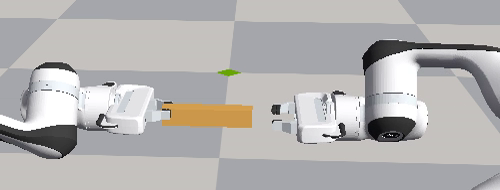
\includegraphics[width=0.49\columnwidth]{figures/frame_a.png}};
\node[inner sep=0,right=0.01\columnwidth of a] (b) {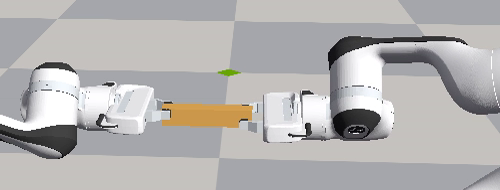
\includegraphics[width=0.49\columnwidth]{figures/frame_b.png}};
\node[inner sep=0,below=0.01\columnwidth of a] (c) {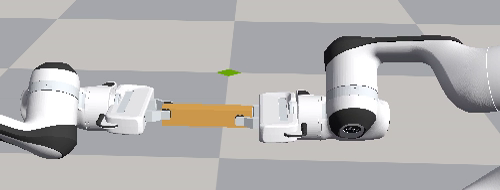
\includegraphics[width=0.49\columnwidth]{figures/frame_c.png}};
\node[inner sep=0,right=0.01\columnwidth of c] (d) {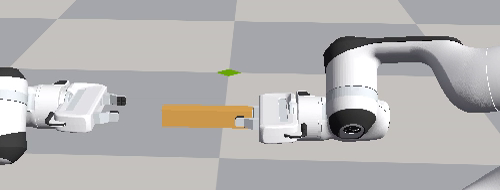
\includegraphics[width=0.49\columnwidth]{figures/frame_d.png}};
\foreach \n/\t in {a/(a) 1.0\,s, b/(b) 2.0\,s, c/(c) 2.9\,s, d/(d) 4.8\,s}
  \node[anchor=north west,fill=white,fill opacity=0.8,text opacity=1,inner sep=1.5pt,font=\footnotesize] at (\n.north west) {\t};
\end{tikzpicture}
\caption{A successful held-out handover with an unknown in-grasp offset ($+15$\,mm along the bar, 10\,mm
vertically) under calibrated geometry.
(a)~The receiver (right) approaches the bar held by the giver (left). (b)~It closes on the estimated grasp point.
(c)~Both grippers hold the bar until the receiver's grasp is stable. (d)~The giver has released and retreated; the
receiver holds the bar alone for 2\,s.}
\label{fig:frames}
\end{figure}

Residual reinforcement learning is a natural remedy~\cite{johannink2019residual,silver2018residual}. A nominal
controller provides structure, and a policy trained in simulation learns a bounded correction for what the
controller gets wrong. Learned handover policies have succeeded with dexterous hands~\cite{frau2025handover}, and
residual learning transfers bimanual dexterous skills~\cite{li2025maniptrans}. It is less clear what the learned
correction contributes once the controller already reasons explicitly about geometry and contact, and whether
memory helps the policy infer an object pose that it cannot observe directly.

We study this question in one carefully controlled task. Two Franka Panda arms with parallel-jaw grippers hand over
a rigid bar in Isaac Lab~\cite{mittal2025isaaclab} (\cref{fig:frames}). We compare a scripted nominal controller,
a training-free geometric coordination module, a PPO residual~\cite{schulman2017ppo}, and their combination, under
four regimes of increasing difficulty: (E1) perturbed object pose and release timing; (E2) corrupted object sensing;
(E3) an unknown object offset inside the giver's grasp; and (E4) a physical slip of the object in the giver's
fingers after the controller has estimated that offset. Every regime uses a protocol frozen before evaluation,
fresh held-out cases, matched training budgets, tuned constant-offset controls, and paired bootstrap intervals.

Our contributions are:
\begin{itemize}
\item A simulated two-arm handover with physically produced grasp uncertainty: offsets are settled by finger
contact, and slips are driven by a regulated force against friction, never by teleporting the object.
\item A geometric coordination module (alignment, shared-holding anchor, contact-gated release) with three
grasp-frame estimators (fixed, calibrated, tracking), and residual PPO variants with and without observation history.
\item A controlled comparison across four uncertainty regimes, including a matched factorial ablation that isolates
the source of the largest gain, and mechanism tests of what the learned policies use.
\item The finding that robustness comes from estimating the object pose in the giver's hand. Learned residuals help
a weak controller, behave like constant offsets on a strong one, and show no benefit from memory.
\end{itemize}
Code, raw records, checkpoints and videos are public~\cite{repo2026}.



\section{Related Work}

\textbf{Handover.} Human--robot handover research studies grasp configuration, timing and release
coordination~\cite{ortenzi2021handover,strabala2013handover}. Learning-based work trains dexterous handover policies
that generalize to unseen objects and motion perturbations~\cite{frau2025handover} and benchmarks bimanual
dexterous skills, including handover, with reinforcement learning~\cite{chen2022bidexhands}. We use parallel-jaw
grippers and isolate the geometric part of the problem: where the object is in the giver's grasp and when the giver
may release.

\textbf{Residual learning.} Residual reinforcement learning adds a learned correction to a hand-designed
controller, which improves sample efficiency and keeps the controller's structure~\cite{johannink2019residual,
silver2018residual}. Residual physics similarly corrects an analytic model with a learned term~\cite{zeng2020tossingbot},
and ManipTrans uses residual learning to transfer human bimanual demonstrations~\cite{li2025maniptrans}. We test
residuals against strong training-free baselines and constant offsets, which separates state-dependent correction
from a learned bias.

\textbf{Robustness and memory.} Randomizing perception and dynamics during training makes simulated policies
robust~\cite{tobin2017domain,peng2018dynamics}, and stacking recent observations lets a policy infer hidden state
such as velocity~\cite{mnih2015dqn}. We test whether a stacked history lets a residual infer a hidden in-grasp
offset and its change, and we compare it with input-size and order-shuffling controls.

\section{Task and Methods}

\subsection{Handover Task}
\label{sec:task}

Two Franka Panda arms face each other across a table (\cref{fig:frames}). The giver initially holds an
$18\times3.5\times3.5$\,cm, 0.15\,kg rigid bar by one end; the receiver must grasp the other end. Physics runs at
120\,Hz in PhysX (Isaac Sim 6.2, Isaac Lab 3.0~\cite{mittal2025isaaclab}) and control at 20\,Hz through
differential inverse kinematics with fixed commanded hand orientations. The nominal schedule reaches pre-grasp at
1.0\,s, closes the receiver from 2.0 to 2.8\,s, and requests the giver's release at 2.8\,s (plus a perturbation).
An episode succeeds if, within 8\,s, the receiver alone holds the bar for 2\,s: giver open and out of contact, no
table support, above the drop height and with low relative speed. A prohibited collision (receiver fingers against
the bar end or other bodies), a drop, a release timeout or the time limit ends the episode as a failure. Resets
that fail validation count as failures in the all-scheduled denominator.

\subsection{Geometric Coordination}

The geometric module runs without training and has three parts (\cref{fig:arch}).

\textbf{Alignment.} Before stable receiver contact, the receiver target is
\begin{equation}
p_{\text{cmd}} = p_{\text{nom}}(t) + \operatorname{clip}\!\big(k\,(g(\hat p) - p_{\text{nom}}(t)),\,\pm b\big) + r_t,
\label{eq:align}
\end{equation}
where $p_{\text{nom}}$ is the nominal receiver trajectory, $g(\hat p)$ is the grasp point implied by the bar estimate
$\hat p$, $b$ is a per-axis alignment bound (15 or 25\,mm), and $r_t$ is the optional learned residual.

\textbf{Shared-holding anchor.} Once the receiver is stable (both fingers above 0.2\,N, relative linear speed below
0.03\,m/s and angular speed below 0.5\,rad/s for 0.15\,s), the receiver target is anchored at its actual grasp
position and the residual may move it at most 1\,cm per axis.

\textbf{Contact-gated release.} The giver opens only when the release has been requested \emph{and} the receiver is
stable. If stability does not arrive within 1\,s of the request, the episode ends as a release timeout.

\textbf{Grasp-frame estimators.} The bar position $\hat p$ comes from the giver's kinematics. With the giver's
measured tool pose $(p_g, R_g)$ and nominal grasp vector $c_0$, the \emph{fixed} estimate is
$\hat p = p_g + R_g c_0$; an unknown in-grasp offset $\delta$ becomes an equal, undetected error. The
\emph{calibrated} estimate averages the corrupted bar measurement $y_t$ against the kinematic prediction during the
first 0.5\,s (10 frames) while the giver holds the bar,
\begin{equation}
\hat\delta = \tfrac{1}{10}\textstyle\sum_{t=1}^{10} R_g^{\top}\big(y_t - p_g - R_g c_0\big),\qquad
\hat p = p_g + R_g (c_0 + \hat\delta),
\end{equation}
which removes the offset and averages measurement noise, but keeps sensor bias. The \emph{tracking} estimate keeps
updating $\hat\delta$ after the window with an exponential moving average (weight $\beta = 0.05$ per fresh frame)
while both giver fingers hold the bar. During the 0.5\,s window the receiver is still far from the bar, so no
method's timing changes.

\begin{figure}[t]
\centering
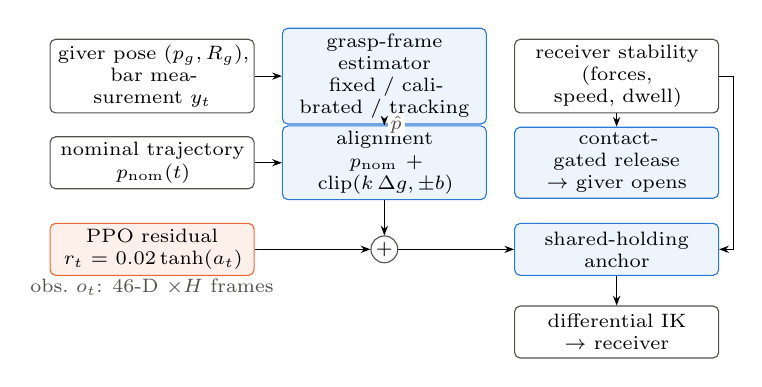
\begin{tikzpicture}[
  font=\scriptsize, >={Stealth[length=3.5pt]},
  blk/.style={draw=vink, rounded corners=2pt, align=center, inner sep=2pt, minimum height=0.66cm,
              text width=2.45cm, fill=white},
  geo/.style={blk, fill=vblue!8, draw=vblue},
  lrn/.style={blk, fill=vorange!10, draw=vorange},
  sum/.style={circle, draw=vink, inner sep=0pt, minimum size=0.34cm, fill=white},
  lab/.style={font=\scriptsize, text=vink, fill=white, inner sep=1pt}]
\node[blk] (sens) at (0,0) {giver pose $(p_g,R_g)$,\\ bar measurement $y_t$};
\node[geo] (est) at (2.95,0) {grasp-frame estimator\\ fixed / calibrated / tracking};
\node[blk] (stab) at (5.9,0) {receiver stability\\ (forces, speed, dwell)};
\node[blk] (nom) at (0,-1.1) {nominal trajectory\\ $p_{\text{nom}}(t)$};
\node[geo] (align) at (2.95,-1.1) {alignment\\ $p_{\text{nom}}+\operatorname{clip}(k\,\Delta g,\pm b)$};
\node[geo] (gate) at (5.9,-1.1) {contact-gated release\\ $\to$ giver opens};
\node[lrn] (ppo) at (0,-2.2) {PPO residual\\ $r_t=0.02\tanh(a_t)$};
\node[sum] (s) at (2.95,-2.2) {$+$};
\node[geo] (anc) at (5.9,-2.2) {shared-holding\\ anchor};
\node[blk] (ik) at (5.9,-3.25) {differential IK\\ $\to$ receiver};
\node[lab, anchor=north] at (ppo.south) {obs.\ $o_t$: 46-D $\times H$ frames};
\draw[->] (sens) -- (est);
\draw[->] (est) -- node[lab, right=1pt]{$\hat p$} (align);
\draw[->] (nom) -- (align);
\draw[->] (align) -- (s);
\draw[->] (ppo) -- (s);
\draw[->] (s) -- (anc);
\draw[->] (anc) -- (ik);
\draw[->] (stab) -- (gate);
\draw[->] (stab.east) -- ++(0.18,0) |- (anc.east);
\end{tikzpicture}
\caption{Controller structure. Blue blocks form the training-free geometric module; the orange block is the
optional learned residual. The grasp-frame estimator supplies the bar position $\hat p$; alignment uses
$\Delta g = g(\hat p) - p_{\text{nom}}$.}
\label{fig:arch}
\end{figure}

\subsection{Residual Policy}

The residual $r_t = 0.02\tanh(a_t)$\,m per axis is added to the receiver target (\cref{eq:align}); orientation
targets stay fixed. The 46-D observation contains the grasp-point error, the orientation error, the bar's linear and
angular velocity relative to the receiver, the giver--receiver offset, both finger widths, four finger contact
forces, receiver joint positions and velocities, the nominal tracking error, normalized time, the previous residual
and a four-way contact phase. The bar position enters only through the controller's estimate; no policy sees the
true offset, slip or case label. The reward is
\begin{equation*}
r = r_{\text{approach}} + 2\,\mathbf{1}_{\text{hold}}\,\Delta t + R_{\text{term}}
  - 0.5\,\Delta t\,\big(\lVert r_t/b_r\rVert^2 + \lVert \Delta r_t/b_r\rVert^2\big),
\end{equation*}
with a shaped approach term $(1-\tanh(d/0.02))\,\Delta t$ before release, terminal rewards $+10$ (success), $-5$
(drop or collision) and $-2$ (release timeout), and $b_r = 2$\,cm.

We train with RSL-RL PPO~\cite{schwarke2025rslrl,schulman2017ppo}: actor and critic MLPs with two 128-unit ELU layers,
observation normalization, initial action std 0.5, 32 steps per environment, 5 epochs of 4 minibatches, adaptive
learning rate ($3\times10^{-4}$, target KL 0.01), $\gamma=0.99$, $\lambda=0.95$, clip 0.2 and entropy 0.002. Each run
uses 10,027,008 transitions, with a curriculum that widens the perturbations. Profiles differ only in their inputs or
parent controller: \emph{feed-forward} (current frame), \emph{history} (four stacked frames; five in E2), \emph{repeated frame}
(the current frame copied four times, an input-size control) and \emph{residual-only} (history on the nominal
controller, no geometry). Every profile uses five training seeds (three in E1). A checkpoint is selected on separate
validation cases by success, then unsafe events, then residual magnitude; the untrained step-0 checkpoint is never
eligible. We report selected and final checkpoints.

\subsection{Uncertainty Regimes}
\label{sec:regimes}

\textbf{E1, pose and timing.} The bar's start position is perturbed per axis and the release request is moved
earlier or later (training up to $\pm2$\,cm and $\pm0.30$\,s; extrapolation up to $\pm3$\,cm and $\pm0.45$\,s).

\textbf{E2, sensing.} The bar translation measurement has a per-episode bias, per-step noise and a delay of up to
several control steps. Orientation, proprioception and contacts remain measured.

\textbf{E3, unknown in-grasp offset.} During reset the bar is pinned at a shifted pose while the giver closes at its
unshifted hold pose; the pin is then removed and only finger contact holds the bar. A probe found the physically
stable region $x\in[-7,+15]$\,mm along the bar and $z\in[-15,+15]$\,mm vertically (fingers re-center $y$). Training
covers $x\in[-5,+15]$, $z\in[-10,+10]$\,mm. Test conditions include fixed offsets up to 15\,mm, a mixed in-distribution
condition (\cond{mixed\_id}, offsets plus sensor corruption), a harder mixture (\cond{mixed\_ood}) and the palm-side
boundary $x=-7$\,mm.

\textbf{E4, in-grasp slip.} After the calibration window, an external force along the bar axis, regulated by a PID
loop (capped at 90\,N), drives the bar's in-grasp displacement along a minimum-jerk profile over 0.25\,s, holds it for
0.1\,s and then vanishes. The giver keeps its normal squeeze, so friction alone holds the bar. Onsets are uniform in
$[0.7, 1.4]$\,s, so every slip ends before the receiver grasps at 2.0\,s. A feasibility probe showed that only
slides toward the receiver of up to 8\,mm are physically reliable (\cref{fig:slip}). Slides toward the palm make the
bar sag and were never valid beyond $-2.5$\,mm (0 of 476 development episodes), and 8--10\,mm slides toward the
receiver were valid in only 93.7\% of episodes.
The conditions therefore use slides of $0$ to $+8$\,mm. A slip that misses its target by more than 1.5\,mm ends the
episode as \emph{invalid} and counts as a failure for every method.

\begin{figure}[t]
\centering
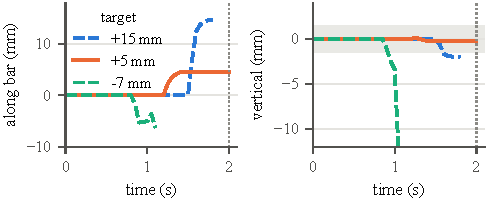
\includegraphics[width=\columnwidth]{figures/slip_mechanism.pdf}
\caption{Physical slip in the development probe: in-grasp displacement of the bar after slip onset, along the bar
(left) and vertically (right). The $+5$\,mm slide tracks its target and stays inside the 1.5\,mm validity band (gray).
The $+15$\,mm slide sags by 2\,mm, and the $-7$\,mm slide toward the giver's palm sags by more than 10\,mm. Dotted line:
receiver grasp at 2.0\,s.}
\label{fig:slip}
\end{figure}

\subsection{Evaluation Protocol}

Each regime was preregistered: suites, seeds, baselines, selection rules and the analysis script were frozen in a
tagged commit before any final evaluation. Final suites use fresh base cases (200 per condition) disjoint from
training, development and validation. Every method runs on the same cases. Differences are estimated with a paired
bootstrap over training seeds and base cases (10,000 draws). Each regime has two primary contrasts with Bonferroni
97.5\% intervals; a superiority claim requires the lower bound to exceed zero. All other comparisons are exploratory
and use 95\% intervals. These rules came from an initial study of the same task, in which geometry was decisive
but checkpoint selection chose the untrained step-0 policy in 8 of 9 runs; such a result cannot show whether training
helped. Every later regime therefore excludes step 0 from selection, initializes the actor with zero mean, and
reports the untrained policy as a separate control. Constant-offset baselines are tuned on development cases with the same bound and
composition as the residual. Repeat evaluations in a second process matched all terminal outcomes in E3 (2,160/2,160), in the E3
ablation (4,800/4,800) and in E4 (12,600/12,600).

Before each freeze, simulator checks guarded the comparisons. Perturbing the privileged tensors (true offset and
achieved offset) at every step left every traced controller quantity bit-identical, so no controller reads hidden
state. In E3, the untrained (zero-mean) checkpoint of every profile reproduced its parent controller on all 72 checked
cases.
Negative controls (no receiver, a giver that never releases, a table that supports the bar) produced no success, and
a no-slip case with the slip mechanism enabled was bitwise identical to the mechanism disabled. One E4 training run
of 10M transitions takes about 21 minutes on one A100 GPU; E4 and the ablation together used 9.49 GPU-hours,
including failed jobs and verification.

\section{Results}

\subsection{E1: Geometry Solves Pose and Timing; Residuals Help Only Without It}

\Cref{tab:e1} shows the held-out E1 suite (2,400 cases, 12 conditions). The residual policy raises the nominal
controller from 65.2\% to 82.6\% (+17.4\pp{} \ci{+15.9}{+19.0}) and beats a tuned constant on the nominal controller
by +13.3\pp{} \ci{+12.0}{+14.7}; its correction tracks the object offset. Geometry reaches 96.5\%. On top of geometry,
the combined policy reaches 96.1\% ($-0.4$\pp{} \ci{-0.8}{-0.2}), and geometry with a tuned 10\,mm constant reaches
99.2\%. The trained combined residuals output an almost state-independent offset of $-1$ to $-2.5$\,mm along the
approach axis (across-case spread $\le 0.6$\,mm), in the opposite direction to the useful constant. Removing the
explicit contact-phase input changes nothing ($-0.2$\pp{} \ci{-0.6}{+0.2}).

A factorial ablation of the geometric module on the same suite attributes the gain mostly to alignment
(+24.0\pp{} \ci{+22.5}{+25.6} at a 1.5\,cm bound) and to the release gate (+7.3\pp{} \ci{+6.5}{+8.2}); the anchor
contributes nothing measurable ($-0.1$\pp). The gate matters most where alignment is imperfect: given alignment, it
adds +25.5\pp{} on $\pm3$\,cm cases at a 1\,cm bound.

\begin{table}[t]
\centering
\caption{E1 held-out success (\%) by perturbation group. Learned rows average three seeds (selected checkpoints).}
\label{tab:e1}
\setlength{\tabcolsep}{4.5pt}
\begin{tabular}{@{}lrrrr@{}}
\toprule
Controller & inner & $\pm2$\,cm & $\pm3$\,cm & all \\
\midrule
Nominal & 96.0 & 50.0 & 18.8 & 65.2 \\
Nominal + residual PPO & 99.9 & 85.5 & 45.2 & 82.6 \\
Geometry (1.5\,cm bound) & 100.0 & 100.0 & 86.2 & 96.5 \\
Geometry + residual PPO & 100.0 & 100.0 & 84.4 & 96.1 \\
Geometry + 10\,mm constant & 100.0 & 100.0 & \textbf{97.0} & \textbf{99.2} \\
\bottomrule
\end{tabular}
\end{table}

\subsection{E2: A Known Grasp Transform Removes Sensing Errors}

E2 corrupts the bar measurement with a per-episode bias (up to 10\,mm), per-step noise (up to 4\,mm) and a delay
of up to four control steps, over 13 conditions (2,600 held-out cases). Geometry that uses the raw estimate collapses:
it reaches 0.5\% at 2\,mm noise and 0.0\% on the mixed condition, almost entirely by release timeouts. An EMA filter ($\alpha=0.2$) restores robustness to noise but not to a
10\,mm bias (67.5\%), which causes collisions. Delay has no effect in this nearly stationary task. Inferring the bar
from the giver's kinematics and the known grasp transform bypasses the corruption: the strongest baseline and every
selected combined policy reached 100\% in all 13 conditions, so both primary contrasts are exactly zero. The learned
residuals again act as constant offsets: their mean $x$ correction has an intercept of $-2.6$ to $-0.4$\,mm and a
slope of at most 0.008 on the injected sensor bias. Without
geometry, sensing errors erase the residual's E1 advantage: a residual-only history policy reaches 68.7\% on the
mixed condition, against 70.5\% for nominal control ($-1.8$\pp{} \ci{-10.2}{+4.4}). Learning helped the weak
controller only when its state estimate was accurate. The ceiling in E2 rests on one assumption, that the grasp
transform is known; E3 removes it.

\subsection{E3: Calibrating the Grasp Transform Carries the Gain}

\Cref{tab:e3} shows the held-out E3 suite (12 conditions $\times$ 200 cases; 129,600 episodes). The fixed transform
fails when the offset is large: 5.5\% at 15\,mm and 69.5\% on \cond{mixed\_id}. Calibrated geometry reaches 94.5\%
and 98.5\%. The learned residuals sit on top of the calibrated parent. The two primary contrasts on
\cond{mixed\_id}, history minus feed-forward (+0.6\pp{} \ci{+0.0}{+2.1}) and history minus the best constant
(+1.5\pp{} \ci{+0.0}{+3.5}), do not establish superiority: both lower bounds touch zero. At the palm-side boundary
$x=-7$\,mm, outside the training support, the history policy drops to 65.2\%, against 96.5\% for its parent
($-31.3$\pp{} \ci{-43.8}{-18.7}). Restricting to the 189 cases with valid resets for every method gives
$-30.8$\pp{} \ci{-43.6}{-18.2}. A residual-only policy without geometry stays near nominal control. EMA geometry, which filters the raw
measurement and uses no giver reference, is also insensitive to the offset (99.0\% on \cond{mixed\_id}), but it
sees the sensor bias directly and trails calibration on \cond{mixed\_ood} (calibrated minus EMA $+4.0$\pp{}
\ci{0.0}{+8.5}).

\begin{table}[t]
\centering
\caption{E3 held-out success (\%) with an unknown in-grasp offset. Learned rows average five seeds (selected
checkpoints) and use the calibrated parent, except residual-only.}
\label{tab:e3}
\setlength{\tabcolsep}{3.7pt}
\begin{tabular}{@{}lrrrr@{}}
\toprule
Controller & 15\,mm & \cond{mixed\_id} & \cond{mixed\_ood} & $x{=}{-}7$ \\
\midrule
Nominal & 38.5 & 59.5 & 59.0 & 48.0 \\
Fixed geometry & 5.5 & 69.5 & 73.5 & 96.0 \\
EMA geometry (no giver ref.) & 94.0 & 99.0 & 90.5 & 96.0 \\
Calibrated geometry & 94.5 & 98.5 & 94.5 & \textbf{96.5} \\
\quad + feed-forward PPO & 96.5 & 99.4 & 94.5 & 88.2 \\
\quad + history PPO & \textbf{99.1} & \textbf{100.0} & \textbf{97.0} & 65.2 \\
\quad + repeated-frame PPO & 96.2 & 99.5 & 91.3 & 91.2 \\
Residual-only history PPO & 40.3 & 56.3 & 53.7 & 42.3 \\
\bottomrule
\end{tabular}
\end{table}

The E3 baseline comparison changed three settings at once: the reference (fixed to calibrated), an EMA filter on the
measurement ($\alpha$ 1.0 to 0.2) and the alignment bound (15 to 25\,mm). A preregistered $2\times2\times2$
factorial isolates them on 2,400 new held-out cases per configuration (\cref{fig:studya}). With $\alpha=0.2$ and a
25\,mm bound fixed, calibrated minus fixed is +29.5\pp{} \ci{+22.5}{+36.5} on \cond{mixed\_id} and
+93.0\pp{} \ci{+88.5}{+96.5} at 15\,mm (Bonferroni 97.5\% intervals); both contrasts are supported. Averaged over the
other factors, the reference adds +24.8\pp{} on \cond{mixed\_id}, the wider bound adds +3.2\pp{} \ci{+1.3}{+5.3}, and
the filter adds exactly zero. The filter's null effect follows from the controller: with the giver reference active,
the filtered measurement reaches the controller only while the receiver waits at its start pose and after the giver
releases. Across 9,600 paired episodes, all recorded outcomes are identical between $\alpha=1.0$ and $0.2$, and in
traced episodes the executed receiver command never differs. The fixed transform fails by collision: on
\cond{mixed\_id} its failures are prohibited receiver contacts with the bar end, most with the receiver misaligned
by more than 10\,mm at grasp time.

\begin{figure}[t]
\centering
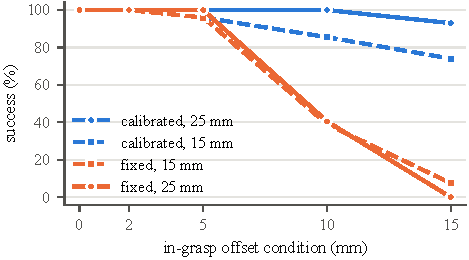
\includegraphics[width=\columnwidth]{figures/study_a_sweep.pdf}
\caption{Matched calibration ablation ($\alpha=0.2$): success versus the in-grasp offset for the fixed and calibrated
grasp transforms at two alignment bounds, 200 held-out cases per point. Calibration keeps success above 93\% at
15\,mm; the fixed transform collapses beyond 5\,mm regardless of the bound.}
\label{fig:studya}
\end{figure}

\subsection{E4: Under Slip, Re-Estimation Matters and Memory Does Not}

A one-shot calibration is correct only while the grasp stays put. E4 slides the bar after the calibration window.
The question is whether a learned residual with history recovers better than (B1) the same residual without history
and (B2) the strongest training-free controller. On development cases, tracking geometry ($\beta=0.05$, 25\,mm bound)
tied with a $+4$\,mm constant offset on success and unsafe events; the preregistered tie-break (smallest total
correction) made tracking the B2 comparator. All learned profiles train with a slip in half of the episodes, on top
of the E3 offsets and sensor corruption.

\Cref{tab:e4} shows the held-out suite (7 conditions $\times$ 200 cases). The slip hurts the one-shot parent: it
falls from 100\% without slip to 90.0\% on \cond{slip\_mixed\_id} and 80.5\% on \cond{slip\_mixed\_ood}. Both
primary contrasts on \cond{slip\_mixed\_id} are small (\cref{fig:contrasts}): history minus feed-forward is
$-1.0$\pp{} \ci{-3.4}{+1.3}, and history minus tracking geometry is +0.9\pp{} \ci{-2.6}{+4.6}. Neither establishes
superiority. Excluding the 23 base cases where any primary arm had an invalid slip leaves the verdict unchanged
(+0.5 and +1.4\pp, both intervals include zero).

\begin{table}[t]
\centering
\caption{E4 held-out success (\%) with a physical in-grasp slip: no slip (static mixed), a $+8$\,mm
slide, and the in- and out-of-distribution slip mixtures. Learned rows pool five seeds
(1,000 episodes per cell). About 6\% of slips are invalid and count as failures for every method.}
\label{tab:e4}
\setlength{\tabcolsep}{4.5pt}
\begin{tabular}{@{}lrrrr@{}}
\toprule
Controller & no slip & $+8$\,mm & mixed ID & mixed OOD \\
\midrule
Nominal & 52.5 & 52.0 & 46.0 & 48.5 \\
Fixed geometry & 69.0 & 77.0 & 52.5 & 59.5 \\
Calibrated (one-shot) & 100.0 & \textbf{97.5} & 90.0 & 80.5 \\
Tracking geometry & 100.0 & 96.5 & 92.0 & 87.5 \\
Calibrated + 4\,mm const. & 100.0 & \textbf{97.5} & \textbf{94.5} & \textbf{92.5} \\
\midrule
\quad + feed-forward PPO & 99.9 & 96.8 & 93.9 & 90.7 \\
\quad + history PPO & 99.0 & 96.9 & 92.9 & 91.4 \\
\quad + repeated-frame PPO & 100.0 & 97.0 & 94.2 & 88.9 \\
\quad + history PPO, final & 63.0 & 78.0 & 63.7 & 59.1 \\
\bottomrule
\end{tabular}
\end{table}

Three simple remedies recover most of the loss. Tracking adds +7.0\pp{} \ci{+3.0}{+11.5} over the one-shot parent on
\cond{slip\_mixed\_ood}. The feed-forward residual adds +3.9\pp{} \ci{+0.9}{+7.3} on \cond{slip\_mixed\_id} and
+10.2\pp{} \ci{+5.9}{+15.0} on \cond{slip\_mixed\_ood}, without any history. A constant +4\,mm offset along the bar
reaches 94.5\% and 92.5\%; because slides go toward the receiver, a bias in that direction pre-compensates them.

\begin{figure}[t]
\centering
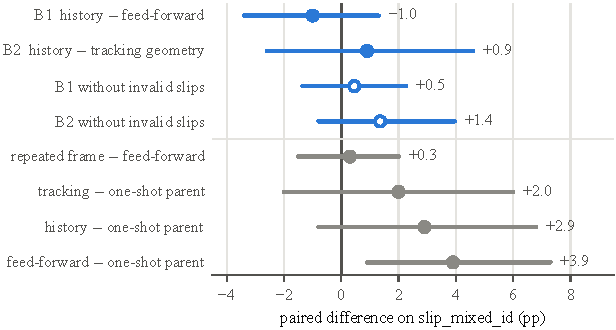
\includegraphics[width=\columnwidth]{figures/slip_contrasts.pdf}
\caption{Paired differences on \cond{slip\_mixed\_id} (selected checkpoints). Blue: the two primary contrasts with
Bonferroni 97.5\% intervals, on all cases (filled) and without invalid slips (hollow). Gray: exploratory contrasts
with 95\% intervals.}
\label{fig:contrasts}
\end{figure}

Training with slip did not hurt the E3 conditions. On the 2,400-case E3 suite without slip, the slip-trained
policies stay within 1.5\pp{} of the E3 policies of the same architecture in most cells and do better at the palm-side
boundary, where the E3 history policies were weakest (history 81.9\% versus 65.2\%; feed-forward 95.3\% versus
88.2\%).

\begin{table}[t]
\centering
\caption{E4 terminal outcomes on the in-distribution slip mixture (\% of scheduled episodes). Invalid slips are decided before
the receiver grasps and count as failures for every method.}
\label{tab:fail}
\setlength{\tabcolsep}{4.5pt}
\begin{tabular}{@{}lrrrr@{}}
\toprule
Controller & success & collision & drop & invalid slip \\
\midrule
Nominal$^{*}$ & 46.0 & 43.0 & 3.5 & 7.0 \\
Fixed geometry & 52.5 & 40.5 & 0.0 & 7.0 \\
Calibrated (one-shot) & 90.0 & 4.5 & 0.0 & 5.5 \\
Tracking geometry & 92.0 & 1.5 & 0.0 & 6.5 \\
Calibrated + 4\,mm const. & 94.5 & 0.0 & 0.0 & 5.5 \\
\quad + feed-forward PPO & 93.9 & 0.7 & 0.0 & 5.4 \\
\quad + history PPO & 92.9 & 0.3 & 0.0 & 6.8 \\
\quad + repeated-frame PPO & 94.2 & 0.0 & 0.0 & 5.8 \\
\bottomrule
\multicolumn{5}{@{}l}{\footnotesize $^{*}$Plus 0.5\% release timeouts.}
\end{tabular}
\end{table}

\textbf{Do the history policies use memory?} On a 60-case mechanism subset of \cond{slip\_mixed\_id}, we re-ran each
selected history policy with its four frames reversed, with the current frame repeated four times, and with its
residual replaced by a constant fitted on its own development records. All five seeds succeed on 52/60 cases in every
variant, with the same terminal outcome on every case; the zero-residual parent succeeds on 48/60. The remaining
failures are the same eight invalid slips. The residual's gain is reproduced by a constant, and the order or presence
of past frames does not matter. In E3, reversing or removing history also changed few outcomes, and a fitted
constant matched or exceeded each history policy.

\textbf{Training stability.} Validation-based selection matters for history policies. Their final checkpoints
degraded in three of five seeds, two of them completely (\cref{fig:seeds}); history final minus selected is
$-29.2$\pp{} \ci{-57.9}{-3.9} on \cond{slip\_mixed\_id}. Feed-forward and repeated-frame final checkpoints stay within
1\pp{} of their selected ones. The same late degradation of history policies appeared in E2 and E3.

\begin{figure}[t]
\centering
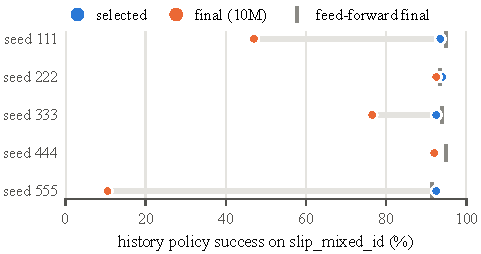
\includegraphics[width=\columnwidth]{figures/history_seeds.pdf}
\caption{Per-seed success of the history policy on \cond{slip\_mixed\_id}: selected checkpoint versus the final
10M-transition checkpoint (seed 444: both 92.0\%). Gray ticks mark feed-forward final checkpoints, which stay stable.}
\label{fig:seeds}
\end{figure}

\subsection{How Controllers Fail}

Across conditions, the dominant failure of every geometry-based controller is a prohibited collision of the receiver
with the bar end, caused by a wrong bar estimate. Contact-gated release does its job: across all 103,200 E3 episodes
of geometry and combined controllers, there are 37 drops and no premature release, while nominal control drops the bar in up to 6.5\% and the residual-only policy in up to 12.1\% of the episodes
of a condition. Conflicting motion during shared holding is rare
(17 of 129,600 E3 episodes, none for a selected combined policy or a geometry baseline). The history policy's
boundary failure in E3 is also a collision problem: at $x=-7$\,mm it collides in 31.2\% of episodes, against 0.5\% for
its parent. In E4 (\cref{tab:fail}), nominal and fixed geometry collide in 43.0\% and 40.5\% of \cond{slip\_mixed\_id}
episodes; the one-shot parent collides in 4.5\%, tracking in 1.5\% and the constant-offset controller in none. For the
strong controllers, almost every remaining failure is an invalid slip (5.4--6.8\%), which caps success near 94\%.
The invalid-slip rate varies slightly between methods because PhysX trajectories depend on the batch layout of the
shared scene; replaying 60 cases at a different batch size changed slip validity in 9 of 120 episodes and nothing
else. Median
completion times of successful E3 episodes are 4.85--4.90\,s for every method on the four main conditions, except EMA
geometry on \cond{mixed\_ood}, where the gate waits longer (5.10\,s).

\section{Discussion}

\textbf{Estimate the grasp, then correct.} Across four regimes, the largest gains came from giving the controller a
better estimate of where the bar sits in the giver's hand: alignment to the estimated grasp point in E1, the giver's
kinematics in E2, a 0.5\,s calibration in E3, and continuous re-estimation in E4. Each is cheap, needs no training,
and carries over across conditions. The learned residual helped when the controller was weak or its estimate was stale,
and in those cases a constant offset or a memoryless policy captured the gain.

\textbf{When the residual helps.} The residual added real, state-dependent value only once: on the nominal
controller in E1, where its correction tracked the object offset and beat the best constant by 13.3\pp. That
correction relied on an accurate bar measurement. With the corrupted sensing of E2, the same kind of policy fell to
the level of the nominal script. On top of geometry, the policy had little error left to correct and converged to a
small constant bias.

\textbf{Why memory did not help.} A stacked history could, in principle, let a policy infer the offset and the slip
from the motion of the bar estimate. In our task, the controller's estimate already contains that information, and
the remaining error is close to a constant bias in a known direction. The mechanism tests confirm that the policies
learned that bias. The history input also made training less stable and reduced robustness outside the training
support, so its cost was larger than its benefit.

\textbf{Design guidance.} Three practices follow from these results. First, give the receiver an estimate of
the object pose in the giver's frame and refresh it while the giver holds the object; a short calibration window and
a slow tracking filter cost no task time. Second, gate the giver's release on measured receiver stability, which
removed drops and premature releases in every regime. Third, evaluate any learned residual against a tuned constant
offset, a shuffled-input control and the untrained parent, and select checkpoints on validation data. Without these
controls, a constant bias or a lucky checkpoint can look like learned, state-dependent correction.

\textbf{Relation to learned handover.} Learned dexterous handover policies infer the object pose from perception
and contact~\cite{frau2025handover}. Our results suggest a division of labor for such systems: an explicit estimate of
the object in the giver's frame, refreshed from kinematics and measurement, plus a learned layer for the errors that
this estimate cannot represent, such as rotational slip or deformation. Residual learning suits that
layer~\cite{johannink2019residual,silver2018residual}, but its value should be measured against the estimator it sits
on, not against a nominal script.

\textbf{Limitations.} All results are in simulation with one rigid bar, fixed physical parameters, commanded
orientations and synthetic sensing. Calibration inherits the sensor bias, and it
assumes the grasp stays fixed during the 0.5\,s window. The slip model covers one direction and up to 8\,mm, and its invalid-slip rate
depends on PhysX batch layout. The strong baselines are near the ceiling on several conditions, which limits the room
for any learned improvement. Five training seeds give limited information about optimization variability. Tasks with
rotational slip, deformable objects, vision or dexterous hands may favor learned or memory-based correction.

\section{Conclusion}

We studied when residual reinforcement learning improves a geometric controller for bimanual handover. In a
controlled two-arm task with preregistered held-out tests, alignment and contact-gated release removed drops and
premature releases, and the success of every controller depended on its estimate of the object pose in the giver's
grasp. Calibrating that estimate raised success by 29.5\pp{} with an unknown offset, and re-estimating it, or adding a
memoryless residual, recovered most of the loss from a slip. Observation history gave no measurable benefit and
degraded late in training. For handover with parallel-jaw grippers, the first priority is to estimate where the
object is in the giver's hand; learned correction is a useful second layer. Future work will test rotational slip,
varied objects and friction, and transfer to hardware.

\section*{Disclosure}
This was an individual course project. Implementation, experiments, analysis and drafting used an AI coding
assistant (Anthropic Claude via Claude Code) under the author's direction. All numbers come from recorded simulator
runs; every table and figure is regenerated from the released raw records by scripts in the repository~\cite{repo2026}.

\bibliographystyle{IEEEtran}
\bibliography{refs}

\end{document}
